\documentclass{ctexart}
\usepackage{amsmath}
% Warning: amsthm should be imported after amsmath
\usepackage{amsthm}
\usepackage{multicol}
\usepackage{pdfpages}
\newtheorem{thm}{Theorem}
\newtheorem{defn}{Definition}
\newtheorem{refl}{Reflection}
\newtheorem{prob}{Problem}
\renewcommand*{\proofname}{Solution}
\allowdisplaybreaks
\newcommand{\sint}{\frac{\sqrt{3}}{2}}
\newcommand{\half}{\frac{1}{2}}
\newcommand{\qurad}{\frac{1}{4}}
\newcommand{\pare}[1]{\left(#1\right)}
\newcommand{\Quad}{Ax^2 + By^2 + Cxy + Dx +Ey + F = 0}
\newcommand{\degr}{^\circ}
\begin{document}
\section{Conic Curves}
\begin{defn}
For a quadratic curve
\[ \Quad, \]
the discriminant is defined as $\Delta = B^2-4AC$.
\end{defn}
\begin{thm}
The discriminant catagories the quadratic curve as:
\begin{enumerate}
\item $\Delta<0$: Ellipse, point or null;
\item $Delta=0$: Parabola, line, parallel line pair or null;
\item $Delta>0$: Hyperbola or crossing lines.
\end{enumerate}
\end{thm}
\begin{thm}
The equation of tangen line at $(x_0, y_0)$ is
\[ Ax_0x + By_0y + C\frac{x_0 y + y_0 x}{2} + D\frac{x+x_0}{2} + E\frac{y+y_0}{2} + F=0. \]
\end{thm}
\begin{thm}
The equation of the chord crossing the two tangent points is
\[ Ax_0x + By_0y + C\frac{x_0 y + y_0 x}{2} + D\frac{x+x_0}{2} + E\frac{y+y_0}{2} + F=0. \]
\end{thm}
\begin{thm}
The equation of the intersection of the two tangent lines crossing the two intersection points of a chord is
\[ Ax_0x + By_0y + C\frac{x_0 y + y_0 x}{2} + D\frac{x+x_0}{2} + E\frac{y+y_0}{2} + F=0. \]
\end{thm}


\section{General Geometry}
\begin{refl}
为求解关于三角形之问题,可借助
\begin{enumerate}
\item 正弦定理获得正弦与边之关系;
\item 余弦定理获得余弦与相应边之关系;
\item 余弦定理将边的平方降次;
\end{enumerate}
必要时,应组合上述反射。
\end{refl}

\begin{figure}[!h]
\centering
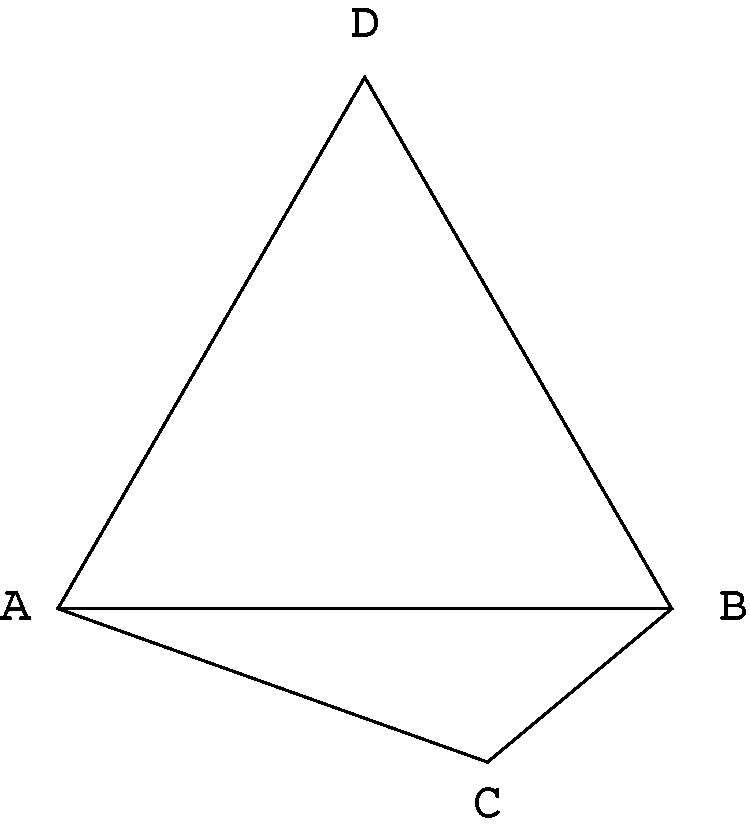
\includegraphics[page=1,width=.5\linewidth]{Triangle1.pdf}
\caption{}
\end{figure}

\begin{prob}
Given $AC=4$,$BC=2$, $\Delta ABD$ is a equilateral triangle. Evaluate the maxium of $S_{\Delta ACD}$.
\end{prob}
\begin{proof}
With \[ a^2 = 20 - 16 \cos C,\quad 4 = a^2 + 16 - 8a\cos A, \]
and \[ a \sin A = 2 \sin C, \]
\begingroup
\begin{align*}
S = 2a\sin DAC &= 2a \pare{ \sin 60\degr \cos A + \cos 60 \degr \sin A } \\
&= 2a \pare{\sint \frac{a^2 + 12}{8a} + \half \frac{2\sin C}{a}} \\
&= \sint\qurad\pare{a^2+12} + 2\sin C \\
&= \sint\qurad\pare{32 - 16 \cos C} + 2\sin C \le 4 + 4\sqrt{3}. \qedhere
\end{align*}
\end{proof}
\endgroup


\section{Functions and Analysis}
\begin{refl}
To compare two numbers involving a transcendental expression, one may construct a function whose variable substitute the transcendental and evaluate its minimum value. Where duplicated occurrence may give some clues to decide the position of the variable.
\end{refl}
\begin{prob}
Compare the following couples of numbers:
\begin{multicols}{2}
\begin{enumerate}
\item $\log 3, \sqrt{3}\log 2$
\item $\log\pi, \sqrt{\frac{\pi}{e}}$
\item $2^{\sqrt{15}}, 15$
\item $3e\ln 2, 4\sqrt 2$
\end{enumerate}
\end{multicols}
\end{prob}
\begin{proof}
With \[ f = \frac{\log x}{x}, \]
which attains its maximum value at $x=e$ when $f\pare{x} = 1/e$ and is monotone increasing for $x<e$, one may reduce the first comparison to
\[ \frac{\log \sqrt{3}}{\sqrt{3}}, \frac{\log 2}{2}, \]
whose relative sizes are obvious with the $f$.

The second one may amount to compare
\[ \frac{\log \sqrt{\pi}}{\sqrt{\pi}}, \frac{\log e}{\sqrt{e}}, \]
which is again obvious with the argument above. A similar argument applies to the rest cases.
\end{proof}
\end{document}